% Copyright 2006 by Till Tantau
%
% This file may be distributed and/or modified
%
% 1. under the LaTeX Project Public License and/or
% 2. under the GNU Free Documentation License.
%
% See the file doc/generic/pgf/licenses/LICENSE for more details.


\section{Matrix Library}

\begin{tikzlibrary}{matrix}
    This library package defines additional styles and options for creating
    matrices.
\end{tikzlibrary}
%
\begin{codeexample}[setup code,hidden]
    \usetikzlibrary{matrix}
\end{codeexample}


\subsection{Matrices of Nodes}

A \emph{matrix of nodes} is a \tikzname\ matrix in which each cell contains a
node. In this case it is bothersome having to write |\node{| at the beginning
of each cell and |};| at the end of each cell. The following key simplifies
typesetting such matrices.

\begin{key}{/tikz/matrix of nodes}
    Conceptually, this key adds |\node{| at the beginning and |};| at the end
    of each cell and sets the |anchor| of the node to |base|. Furthermore, it
    adds the option |name| option to each node, where the name is set to
    \meta{matrix name}|-|\meta{row number}|-|\meta{column number}. For
    example, if the matrix has the name |my matrix|, then the node in  the
    upper left cell will get the name |my matrix-1-1|.
    %
\begin{codeexample}[]
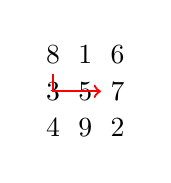
\begin{tikzpicture}
  \matrix (magic) [matrix of nodes]
  {
    8 & 1 & 6 \\
    3 & 5 & 7 \\
    4 & 9 & 2 \\
  };

  \draw[thick,red,->] (magic-1-1) |- (magic-2-3);
\end{tikzpicture}
\end{codeexample}

    You may wish to add options to certain nodes in the matrix. This can be
    achieved in three ways.
    %
    \begin{enumerate}
        \item You can modify, say, the |row 2 column 3| style to pass special
            options to this particular cell.
            %
\begin{codeexample}[]
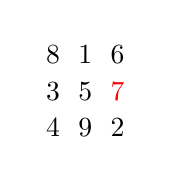
\begin{tikzpicture}[row 2 column 3/.style=red]
  \matrix [matrix of nodes]
  {
    8 & 1 & 6 \\
    3 & 5 & 7 \\
    4 & 9 & 2 \\
  };
\end{tikzpicture}
\end{codeexample}
            %
        \item At the beginning of a cell, you can use a special syntax. If a
            cell starts with a vertical bar, then everything between this bar
            and the next bar is passed on to the |node| command.
            %
{\catcode`\|=12
\begin{codeexample}[]
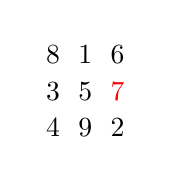
\begin{tikzpicture}
  \matrix [matrix of nodes]
  {
    8 & 1 &         6 \\
    3 & 5 & |[red]| 7 \\
    4 & 9 &         2 \\
  };
\end{tikzpicture}
\end{codeexample}
}
            %
            You can also use an option like \verb!|[red] (seven)|! to give a
            different name to the node.

            Note that the |&| character also takes an optional argument, which
            is an extra column skip.
            %
{\catcode`\|=12
\begin{codeexample}[]
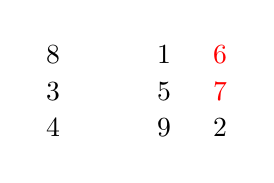
\begin{tikzpicture}
  \matrix [matrix of nodes]
  {
    8 &[1cm] 1 &[3mm] |[red]| 6 \\
    3 &      5 &      |[red]| 7 \\
    4 &      9 &              2 \\
  };
\end{tikzpicture}
\end{codeexample}
}
        \item If your cell starts with a |\path| command or any command that
            expands to |\path|, which includes |\draw|, |\node|, |\fill| and
            others, the |\node{| startup code and the |};| code are suppressed.
            This means that for this particular cell you can provide totally
            different contents.
            %
\begin{codeexample}[]
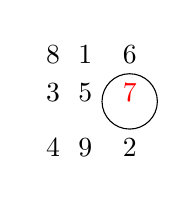
\begin{tikzpicture}
  \matrix [matrix of nodes]
  {
    8 & 1 & 6 \\
    3 & 5 & \node[red]{7}; \draw(0,0) circle(10pt);\\
    4 & 9 & 2 \\
  };
\end{tikzpicture}
\end{codeexample}
    \end{enumerate}
\end{key}

\begin{key}{/tikz/matrix of math nodes}
    This style is almost the same as the previous style, only |$| is added       %$
    at the beginning and at the end of each node, so math mode will be switched
    on in all nodes.
    %
{\catcode`\|=12
\begin{codeexample}[]
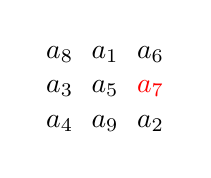
\begin{tikzpicture}
  \matrix [matrix of math nodes]
  {
    a_8 & a_1 &         a_6 \\
    a_3 & a_5 & |[red]| a_7 \\
    a_4 & a_9 &         a_2 \\
  };
\end{tikzpicture}
\end{codeexample}
}
\end{key}

\begin{key}{/tikz/nodes in empty cells=\meta{true or false} (default true)}
    When set to |true|, a node (with empty contents) is put in empty cells.
    Normally, empty cells are just, well, empty. The style can be used together
    with both a |matrix of nodes| and a |matrix of math nodes|.
    %
\begin{codeexample}[]
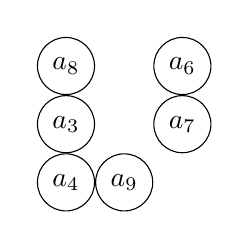
\begin{tikzpicture}
  \matrix [matrix of math nodes,nodes={circle,draw}]
  {
    a_8 &     & a_6 \\
    a_3 &     & a_7 \\
    a_4 & a_9 &     \\
  };
\end{tikzpicture}
\end{codeexample}
    %
\begin{codeexample}[]
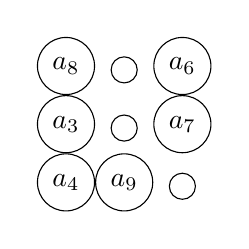
\begin{tikzpicture}
  \matrix [matrix of math nodes,nodes={circle,draw},nodes in empty cells]
  {
    a_8 &     & a_6 \\
    a_3 &     & a_7 \\
    a_4 & a_9 &     \\
  };
\end{tikzpicture}
\end{codeexample}
    %
\end{key}


\subsection{End-of-Lines and End-of-Row Characters in Matrices of Nodes}

Special care must be taken about the usage of the |\\| command inside a matrix
of nodes. The reason is that this character is overloaded in \TeX: On the one
hand, it is used to denote the end of a line in normal text; on the other hand
it is used to denote the end of a row in a matrix. Now, if a matrix contains
node which in turn may have multiple lines, it is unclear which meaning of |\\|
should be used.

This problem arises only when you use the |text width| option of nodes. Suppose
you write a line like
%
\begin{codeexample}[code only]
\matrix [text width=5cm,matrix of nodes]
{
  first row & upper line \\ lower line \\
  second row & hmm \\
};
\end{codeexample}
%
This leaves \TeX\ trying to riddle out how many rows this matrix should have.
Do you want two rows with the upper right cell containing a two-line text. Or
did you mean a three row matrix with the second row having only one cell?

Since \TeX\ is not clairvoyant, the following rules are used:
%
\begin{enumerate}
    \item Inside a matrix, the |\\| command, by default, signals the end of the
        row, not the end of a line in a cell.
    \item However, there is an exception to this rule: If a cell starts with a
        \TeX-group (this is, with |{|), then inside this first group the |\\|
        command retains the meaning of ``end of line'' character. Note that
        this special rule works only for the first group in a cell and this
        group must be at the beginning.
\end{enumerate}

The net effect of these rules is the following: Normally, |\\| is an end-of-row
indicator; if you want to use it as an end-of-line indicator in a cell, just
put the whole cell in curly braces. The following example illustrates the
difference:
%
\begin{codeexample}[]
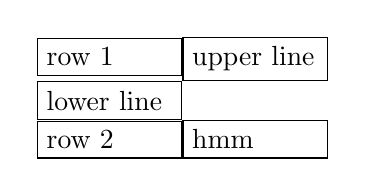
\begin{tikzpicture}
  \matrix [matrix of nodes,nodes={text width=16mm,draw}]
  {
    row 1 & upper line \\ lower line \\
    row 2 & hmm \\
  };
\end{tikzpicture}
\end{codeexample}
\begin{codeexample}[]
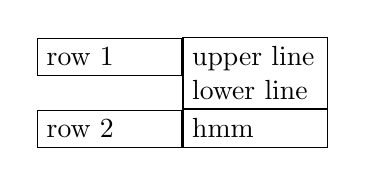
\begin{tikzpicture}
  \matrix [matrix of nodes,nodes={text width=16mm,draw}]
  {
    row 1 & {upper line \\ lower line} \\
    row 2 & hmm \\
  };
\end{tikzpicture}
\end{codeexample}

Note that this system is not fool-proof. If you write things like |a&b{c\\d}\\|
in a matrix of nodes, an error will result (because the second cell did not
start with a brace, so |\\| retained its normal meaning and, thus, the second
cell contained the text |b{c|, which is not balanced with respect to the number
of braces).


\subsection{Delimiters}

Delimiters are parentheses or braces to the left and right of a formula or a
matrix. The matrix library offers options for adding such delimiters to a
matrix. However, delimiters can actually be added to any node that has the
standard anchors |north|, |south|, |north west| and so on. In particular, you
can add delimiters to any |rectangle| box. They are implemented by ``measuring
the height'' of the node and then adding a delimiter of the correct size to the
left or right using some after node magic.

\begin{key}{/tikz/left delimiter=\meta{delimiter}}
    This option can be given to a any node that has the standard anchors
    |north|, |south| and so on. The \meta{delimiter} can be any delimiter that
    is acceptable to \TeX's |\left| command.
    %
\begin{codeexample}[]
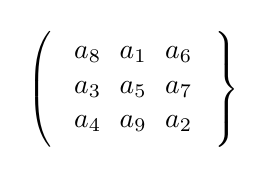
\begin{tikzpicture}
  \matrix [matrix of math nodes,left delimiter=(,right delimiter=\}]
  {
    a_8 & a_1 & a_6 \\
    a_3 & a_5 & a_7 \\
    a_4 & a_9 & a_2 \\
  };
\end{tikzpicture}
\end{codeexample}

\begin{codeexample}[]
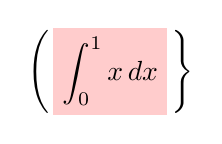
\begin{tikzpicture}
  \node [fill=red!20,left delimiter=(,right delimiter=\}]
    {$\displaystyle\int_0^1 x\,dx$};
\end{tikzpicture}
\end{codeexample}

    \begin{stylekey}{/tikz/every delimiter (initially \normalfont empty)}
        This style is executed for every delimiter. You can use it to shift or
        color delimiters or do whatever.
    \end{stylekey}

    \begin{stylekey}{/tikz/every left delimiter (initially \normalfont empty)}
        This style is additionally executed for every left delimiter.
        %
\begin{codeexample}[]
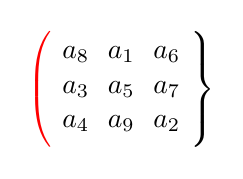
\begin{tikzpicture}
  [every left delimiter/.style={red,xshift=1ex},
   every right delimiter/.style={xshift=-1ex}]
  \matrix [matrix of math nodes,left delimiter=(,right delimiter=\}]
  {
    a_8 & a_1 & a_6 \\
    a_3 & a_5 & a_7 \\
    a_4 & a_9 & a_2 \\
  };
\end{tikzpicture}
\end{codeexample}
    \end{stylekey}
\end{key}

\begin{key}{/tikz/right delimiter=\meta{delimiter}}
    Works as above.
    %
    \begin{stylekey}{/tikz/every right delimiter (initially \normalfont empty)}
        Works as above.
    \end{stylekey}
\end{key}

\begin{key}{/tikz/above delimiter=\meta{delimiter}}
    This option allows you to add a delimiter above the node. It is implemented
    by rotating a left delimiter.
    %
\begin{codeexample}[]
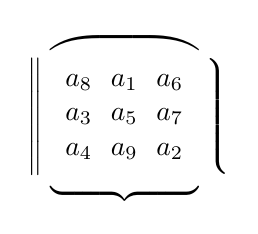
\begin{tikzpicture}
  \matrix [matrix of math nodes,%
           left delimiter=\|,right delimiter=\rmoustache,%
           above delimiter=(,below delimiter=\}]
  {
    a_8 & a_1 & a_6 \\
    a_3 & a_5 & a_7 \\
    a_4 & a_9 & a_2 \\
  };
\end{tikzpicture}
\end{codeexample}

    \begin{stylekey}{/tikz/every above delimiter (initially \normalfont empty)}
        Works as above.
    \end{stylekey}
\end{key}

\begin{key}{/tikz/below delimiter=\meta{delimiter}}
    Works as above.
    \begin{stylekey}{/tikz/every below delimiter (initially \normalfont empty)}
        Works as above.
    \end{stylekey}
\end{key}


%%% Local Variables:
%%% mode: latex
%%% TeX-master: "pgfmanual-pdftex-version"
%%% End:
